\documentclass{article}

\usepackage[left=2.5cm,top=2.5cm,right=2.5cm,bottom=2.5cm,bindingoffset=0.5cm]{geometry}


\usepackage[pdftex]{graphicx}
\usepackage{caption}
\usepackage{subcaption}

\usepackage{amsmath}
\usepackage{amsthm}
\usepackage{amssymb}
\usepackage{mathtools}
\usepackage{commath}
\usepackage{bm}

\usepackage{cleveref}


\usepackage{xcolor}
\usepackage{colortbl}

\usepackage{bm}

\usepackage{url}

\usepackage{listings}
\definecolor{codegreen}{rgb}{0,0.6,0}
\definecolor{codegray}{rgb}{0.5,0.5,0.5}
\definecolor{codepurple}{rgb}{0.58,0,0.82}
\definecolor{backcolour}{rgb}{0.95,0.95,0.92}
 
\lstdefinestyle{mystyle}{
    backgroundcolor=\color{backcolour},   
    commentstyle=\color{codegreen},
    keywordstyle=\color{magenta},
    numberstyle=\tiny\color{codegray},
    stringstyle=\color{codepurple},
    basicstyle=\footnotesize,
    breakatwhitespace=false,         
    breaklines=true,                 
    captionpos=b,                    
    keepspaces=true,                 
    numbers=left,                    
    numbersep=5pt,                  
    showspaces=false,                
    showstringspaces=false,
    showtabs=false,                  
    tabsize=2
}
 
\lstset{style=mystyle}



\title{Inference in the linear model}
\author{Georgios Arampatzis}


\begin{document}

\maketitle


\section{The model}
In this tutorial we will describe how to run the Matlab code for the inference of the parameters in the linear model. We consider the model,
%
\begin{equation}
y = f(x;a,b) = ax + b \, .
\end{equation}
%
We are given $N_d$ data points $\bm{d} = \{y_i,x_i\}_{i=1}^{N_d}$. We consider the statistical model,
%
\begin{equation} \label{eq:model:stat}
y = ax+b + \varepsilon,
\end{equation}
%
where $\varepsilon$ is a random variable that follows normal distribution with mean zeros and standard deviation $\sigma$. We assume that the data $y_i,\, i=1,\ldots,N_d$ are i.i.d samples from the model in \cref{eq:model:stat}.

Set 
%
$$\vartheta=(a,b,\sigma)$$ 
%
the vector of parameters to be inferred. The likelihood of $\bm{d}$ under the assumption  \cref{eq:model:stat} is given by,
%
\begin{equation}
p(\bm{d} | \vartheta) = \mathcal{N} \left( \bm{d} | \bm {\mu}, \Sigma   \right) \, ,
\end{equation}
%
where
%
\begin{equation}
\bm{\mu} = \big(  f(x_1;a,b),\ldots, f(x_{N_d};a,b)  \big)^\top \quad  \mathrm{ and } \quad \Sigma=\sigma^2 I \, .
\end{equation}
%
The log-likelihood is given by,
%
\begin{equation} \label{eq:loglikelihood}
\log p(\bm{d} | \vartheta) = -\frac{1}{2} N_d   \log(2\pi \sigma^2)  -\frac{1}{2 \sigma^2}\sum_{i=1}^{N_d} (y_i - f(x_i;\vartheta))^2 \,.
\end{equation}
%
The derivatives and the Fisher information matrix has been implemented in the provided Matlab functions. The user has to implement the derivatives $\od{}{\vartheta_j}f(x_i,\vartheta)$. 





\section{Running the code}

In order to validate our implementation we will first create synthetic data with known parameters and then infer these parameters. From the root directory (the directory that contains the folders \verb|data| and \verb|engines|), 
%
\begin{lstlisting}[language=Matlab]
	cd data/linear
	make_data
\end{lstlisting}
%
This script will create the file \texttt{data.mat}. Using these data we will infer $a,b$ and $\sigma$.
%
Finally, from the root direcotry run
%
\begin{lstlisting}[language=Matlab]
	addpath(engine/postprocessing/).
\end{lstlisting}







\subsection{Likelihood optimization}
First we can optimize the likelihood function using the CMA-ES algorithm. From the root directory
%
\begin{lstlisting}[language=Matlab]
	cd engine/optimize/
	edit run_linear_CMA.m
\end{lstlisting}
%
%
The important lines in this script are
%
\lstinputlisting[language=Matlab,linerange={12-16}]{../engine/optimize/run_linear_CMA.m}
%
and
%
\lstinputlisting[language=Matlab,linerange={27-28}]{../engine/optimize/run_linear_CMA.m}
%
The \texttt{addpath} command inserts the likelihood functions folder in the search path. In this case the log-likelihood is \verb|linear_loglike_cma| and is located in the folder \verb|../functions/linear/|. This function return the negative of the function \verb|linear_loglike| that implements the log-likelihood as defined in \cref{eq:loglikelihood}.
%
The \texttt{opts.LBounds} and \texttt{opts.UBounds} variables set the search interval for the variables. Here, $a\in[-5,5]$, $b\in[-5,5]$ and $\sigma\in[0,10]$.
Finally, the command
%
%
\lstinputlisting[language=Matlab,linerange={21-21}]{../engine/optimize/run_linear_CMA.m}
%
will start a pool with two workers and run CMA in parallel. If you don't want parallel execution comment out this line. Running the script gives the results,
%
\begin{lstlisting}[language=Matlab]
 Maximum of log-likelihood at:
  a     = 1.867522 
  b     = -1.741286 
  sigma = 1.770017 
\end{lstlisting}










\subsection{Sampling the posterior with BASIS}
From the root directory
%
\begin{lstlisting}[language=Matlab]
	cd engine/sample/
	edit run_linear.m
\end{lstlisting}
%
uncomment the line
%
\begin{lstlisting}[language=Matlab]
	method = 'BASIS'; cov_check = 'NONE';
\end{lstlisting}
%
and run the script. After the end of execution plot the results by running
%
\begin{lstlisting}[language=Matlab]
	plotmatrix_hist(BASIS.theta)
\end{lstlisting}
%
or
%
\begin{lstlisting}[language=Matlab]
	load ../../data/linear/BASIS_NONE_5000.mat
	plotmatrix_hist(out_master.theta)
\end{lstlisting}
%
The results are shown in \cref{fig:basis}.










\subsection{Sampling the posterior with smTMCMC}
First lets examine the function \verb|linear_loglike_smMALA|. From root
\begin{lstlisting}[language=Matlab]
	cd engine/functions/linear/
	edit linear_loglike_smMALA.m
\end{lstlisting}
%
The important lines are 
%
\lstinputlisting[language=Matlab,linerange={21-26}]{../engine/functions/linear/linear_loglike_smMALA.m}
%
Here the variable \verb|dY1| is a row vector that contains the derivative $\od{}{\vartheta_1}f(x_i,\vartheta)$ at the $i$-th position and the variable \verb|dY2| is a row vector that contains the derivative $\od{}{\vartheta_2}f(x_i,\vartheta)$ at the $i$-th position.

In order to run, from the root directory
%
\begin{lstlisting}[language=Matlab]
	cd engine/sample/
	edit run_linear.m
\end{lstlisting}
%
uncomment the line
%
\begin{lstlisting}[language=Matlab]
	method = 'smMALA'; cov_check = 'EIG';
\end{lstlisting}
%
and execute the script.
%
After the end of execution plot the results by running
%
\begin{lstlisting}[language=Matlab]
	plotmatrix_hist(BASIS.theta)
\end{lstlisting}
%
or
%
\begin{lstlisting}[language=Matlab]
	load ../../data/linear/smMALA_EIG_5000.mat
	plotmatrix_hist(out_master.theta)
\end{lstlisting}
%
The results are shown in \cref{fig:smtmcmc}.









\begin{figure}[p]
	\centering
	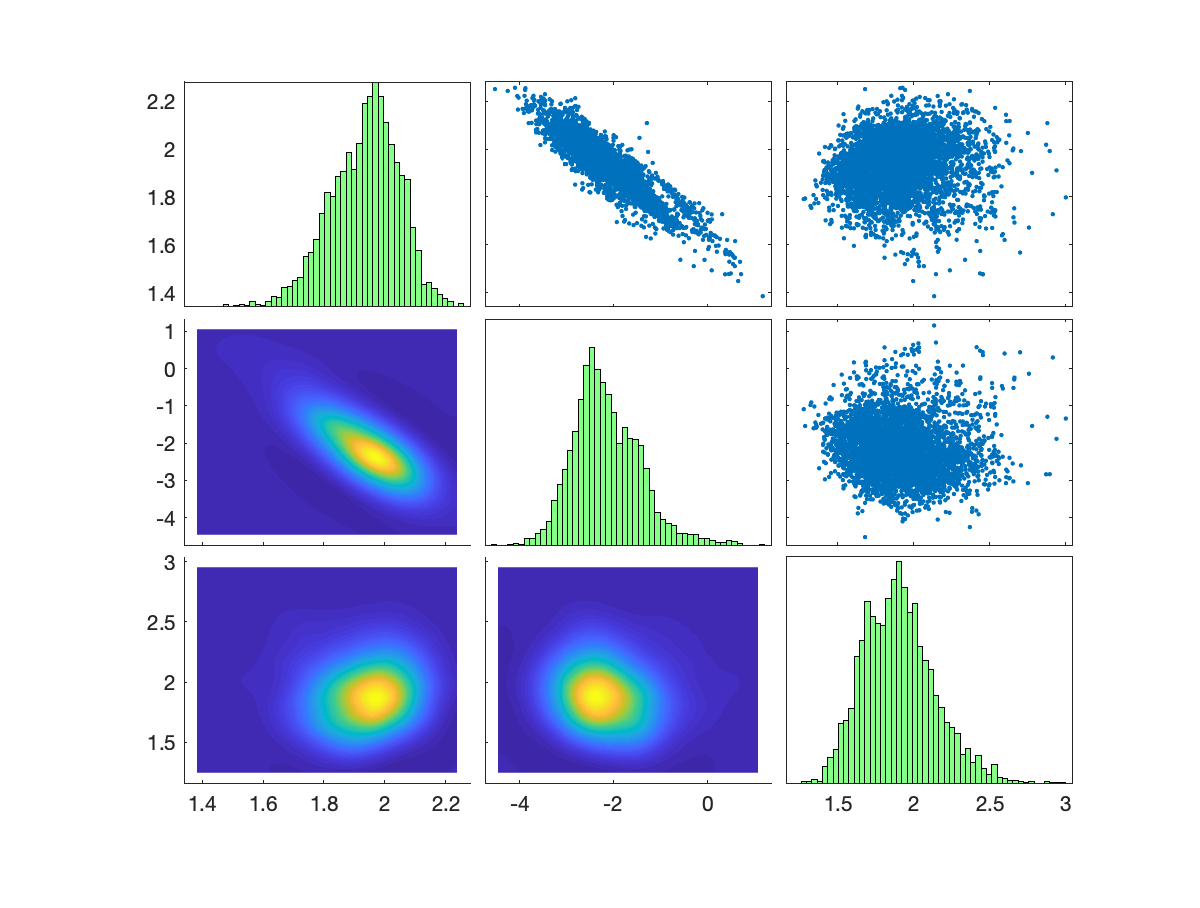
\includegraphics[width=0.8\textwidth]{figures/basis.eps}
	\caption{Results from BASIS.}
	\label{fig:basis}
\end{figure}


\begin{figure}[p]
	\centering
	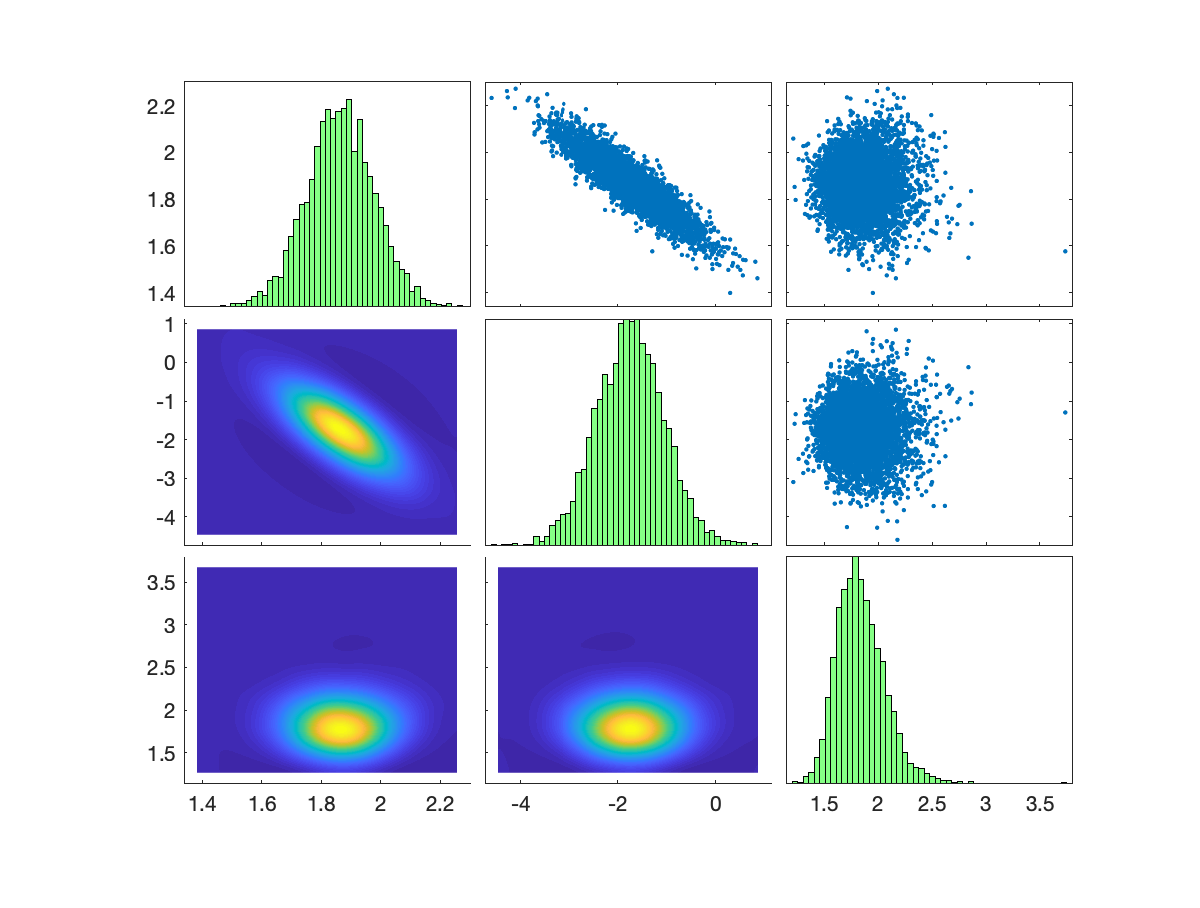
\includegraphics[width=0.8\textwidth]{figures/smtmcmc.eps}
	\caption{Results from smTMCMC.}
	\label{fig:smtmcmc}
\end{figure}






\end{document}



















